\section{Mock samples benchmark}\label{sec:Mock samples}
The beta diversity benchmark for the mock samples is shown in \Cref{fig:mock_human_gut_beta_div_galaxy,fig:mock_soil_beta_div_kraken2}. Given that the taxonomic lineage for the mock sample and Kraken v2 starts at the kingdom rank and concludes at the genus rank, it was necessary to conduct the procedure of adjusting the Galaxy-port lineage, mentioned in \Cref{subsec:mgnifyVSkraken2}. Based on the two plots, it is evident that Galaxy-port (\Cref{fig:mock_human_gut_beta_div_galaxy}) outperformed Kraken v2 (\Cref{fig:mock_soil_beta_div_kraken2}). At each taxonomic rank, the Galaxy-port results displayed on average smaller Bray Curtis and Jaccard distances to the expected taxonomic composition compared to Kraken v2.\par

\begin{figure}[H]
  \centering
  \hfill
  \subfloat{{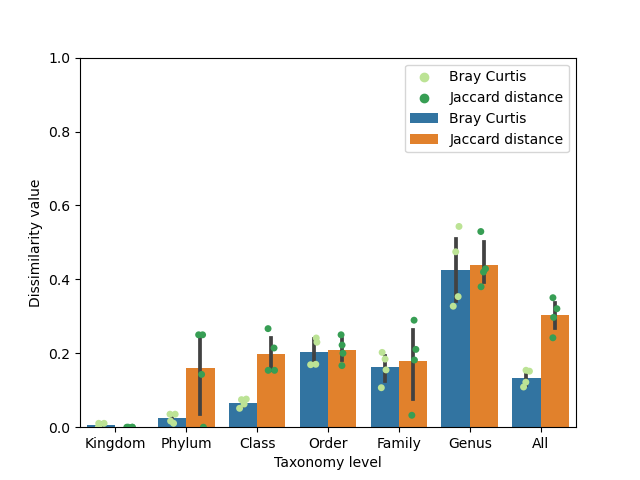
\includegraphics[scale=0.8]{figures/mock_beta_div_expectedVSgalaxy.png} }}%
  \captionof{figure}[Beta diversity-based benchmark. Dissimilarity between expected composition and Galaxy-ported subworkflow, for mock samples]{\textbf{Beta diversity-based benchmark}. Dissimilarity between expected composition and Galaxy-ported subworkflow, for the mock samples (\Cref{subsubsec:mock_samples}). The term 'All' refers to all ranks combined. Bars represent the average dissimilarity values, while individual data points represent the values for each of the individual samples.} \label{fig:mock_human_gut_beta_div_galaxy}%
\end{figure}

\begin{figure}[H]
  \centering
  \hfill
  \subfloat{{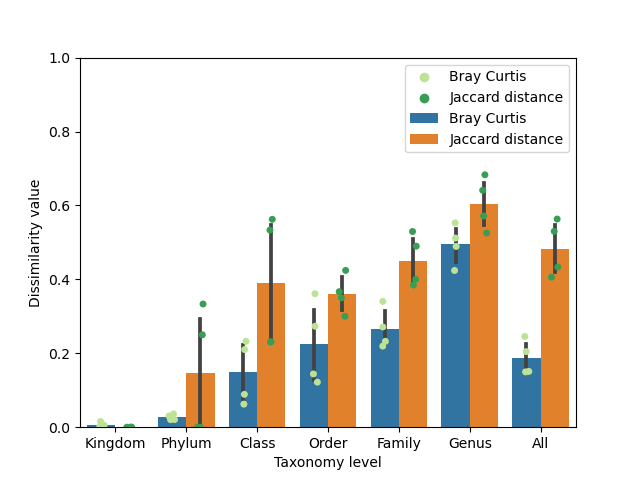
\includegraphics[scale=0.8]{figures/mock_beta_div_expectedVSkraken2.png} }}%
  \captionof{figure}[Beta diversity-based benchmark. Dissimilarity between expected composition and Kraken v2 for mock samples]{\textbf{Beta diversity-based benchmark}. Dissimilarity between expected composition and Kraken v2, for the mock samples (\Cref{subsubsec:mock_samples}). The term 'All' refers to all ranks combined.Bars represent the average dissimilarity values, while individual data points represent the values for each of the individual samples.} \label{fig:mock_soil_beta_div_kraken2}%
\end{figure}

Regarding the generated genus rank relative abundance plot, taxa in the output of Galaxy-ported and Kraken v2 that are differed from the expected taxonomic composition were excluded. The plot of the relative abundance at the genus rank supports the superior performance of Galaxy-port over Kraken v2. The Galaxy visual representation exhibits smaller gaps in comparison to Kraken v2, which means Kraken v2 had higher relative abundance for unexpected taxa. 


\begin{figure}[H]
  \centering
  \subfloat{{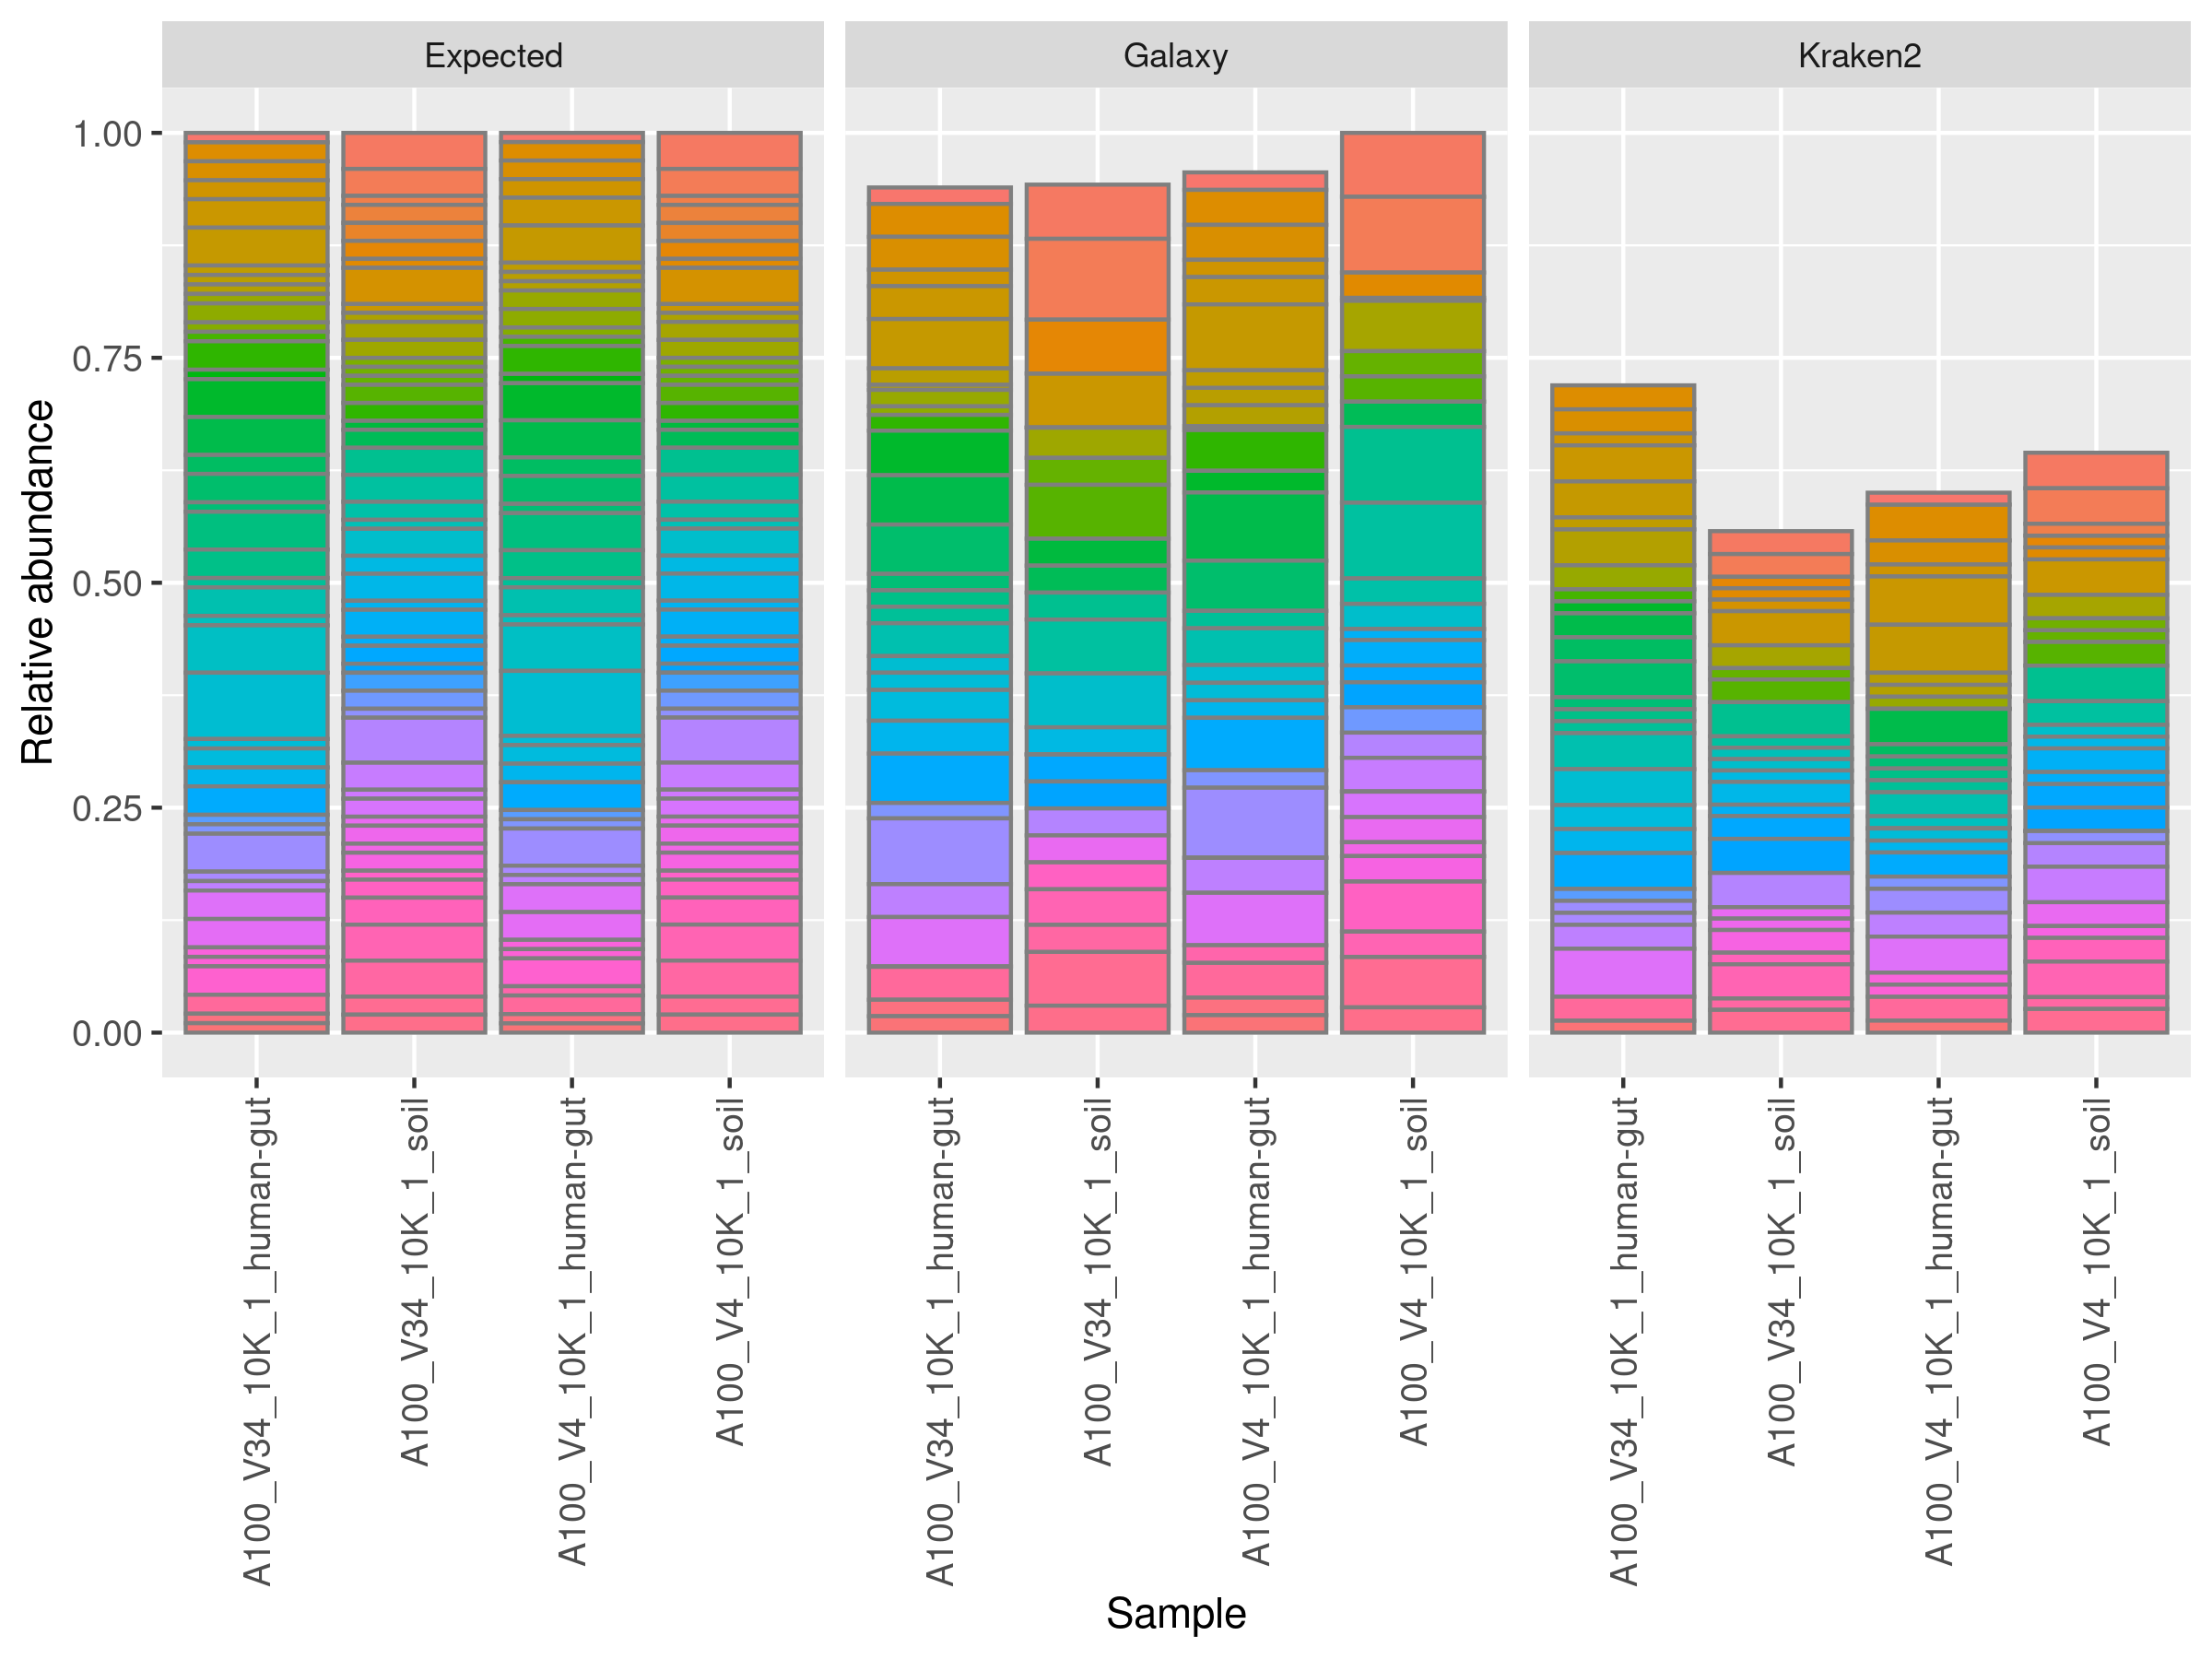
\includegraphics[scale=0.65]{figures/mock_samples_abundance_level_g.png} }}%
  \captionof{figure}[Differences of relative abundance between expected composition, Galaxy-ported subworkflow, and Kraken v2 at genus rank for mock samples]{\textbf{Differences of relative abundance between expected composition, Galaxy-ported subworkflow, and Kraken v2 at genus rank for the mock samples}(\Cref{subsubsec:mock_samples}). Genera that were predicted by Galaxy and Kraken v2 but not present in the expected composition are not shown. The plot legend can be found in the appendix (\Cref{fig:mock_rel_abundance_level_g_legend}).} \label{fig:mock_rel_abundance}%
\end{figure}